\section{Odolnosti proti násilnému vniknutí}

\paragraph{Vytržení dveří}
Jedním ze způsobů~namáhání~mechanizmu~je~vytržení~dveří~z~trezoru.

\subsection{Západka}

\begin{figure}[htbp]
    \centering
    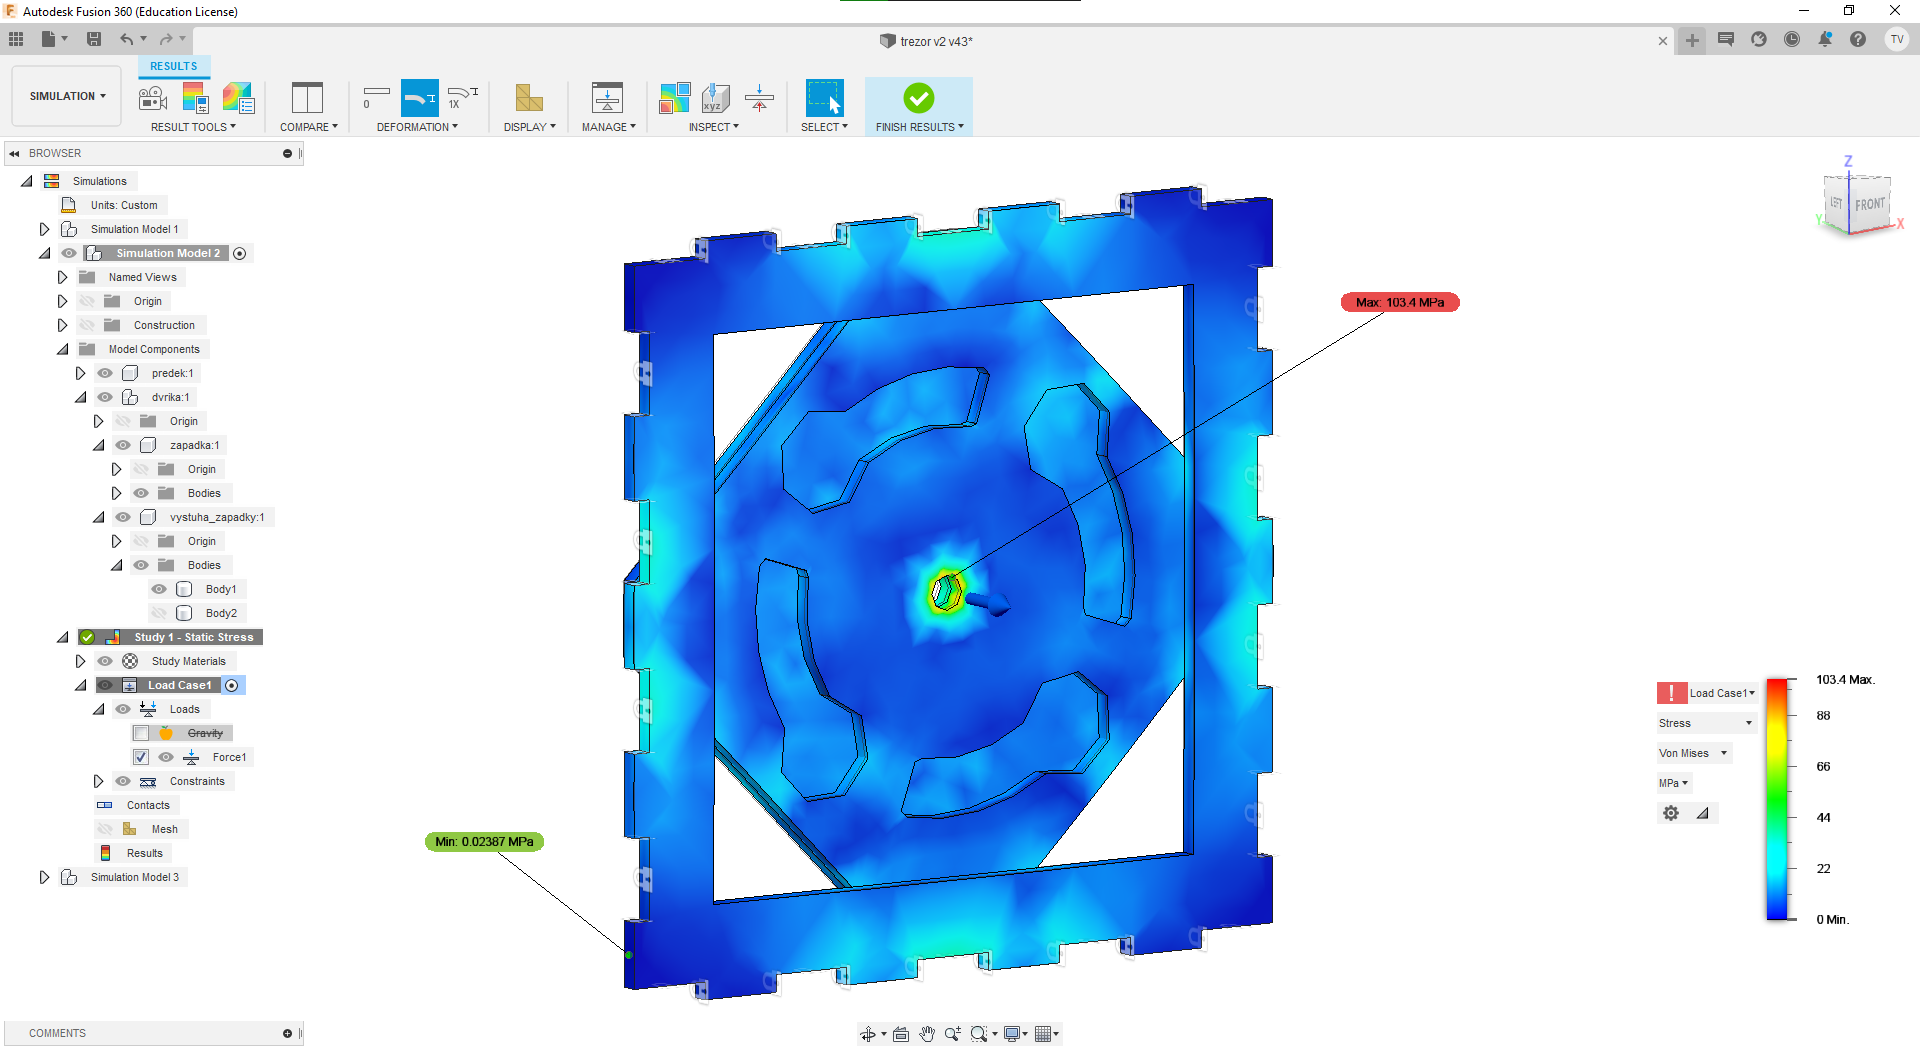
\includegraphics[width=\textwidth]{kapitoly/obrazky/M3/simulace/odolnost_proti_vytrzeni_4kN.png}
    \caption{simulace pokusu o vytržení dveří silou 4 000 N}
    \label{fig:M3-simulace-vytrzeni}
\end{figure}
Ke kompletní simulaci se můžete dostat \href{https://myhub.autodesk360.com/ue2d7aa41/g/shares/SH56a43QTfd62c1cd96843f1e03a0eb48053?viewState=NoIgbgDAdAjCA0IDeAdEAXAngBwKZoC40BlASwFsBXAGwEN1SB7AOzXjVoGdPd1C0ARjABsATlEQItALQBjcbmkAWCMIjSBuWgA5lAM22ilAVgAmMAOyy9%2BBGkYCAVrlnoAkqcIBmAL4gAukA}{zde}
po kliknutí na "Simulation" a "Simulation Model 2". V tabulce napravo se pak můžete přepínat mezi barevným zobrazení několika veličin.

\newpage

\subsection{Kolík}
Při pokusu o vytržení je celá síla přenášena kolíkem.

\(\sigma _M_A_X = 132 MPa\)    ( \href{https://is.mendelu.cz/eknihovna/opory/zobraz_cast.pl?fit_w=1;cast=9190}{dubové dřevo ve směru vláken při vlhkosti 12 \% }) % strana 22 tabulka 2 -> https://www.vutbr.cz/www_base/zav_prace_soubor_verejne.php?file_id=66237

D = 6

\(\sigma _M_A_X = F/S \Rightarrow F = \sigma _M_A_X * S = 132 * (\pi * D^2/4) = 3 732.21 N \) z toho a ze simulace vyplývá že kolík je při namáhání nejslabším členem, přesto že ne o moc.

\paragraph{Otevření bez odemčení}
Dalším způsobem namáhání může být snaha otočit západkou pez zadání správného hesla.

\subparagraph{Západka a kamen}

\begin{figure}[htbp]
    \centering
    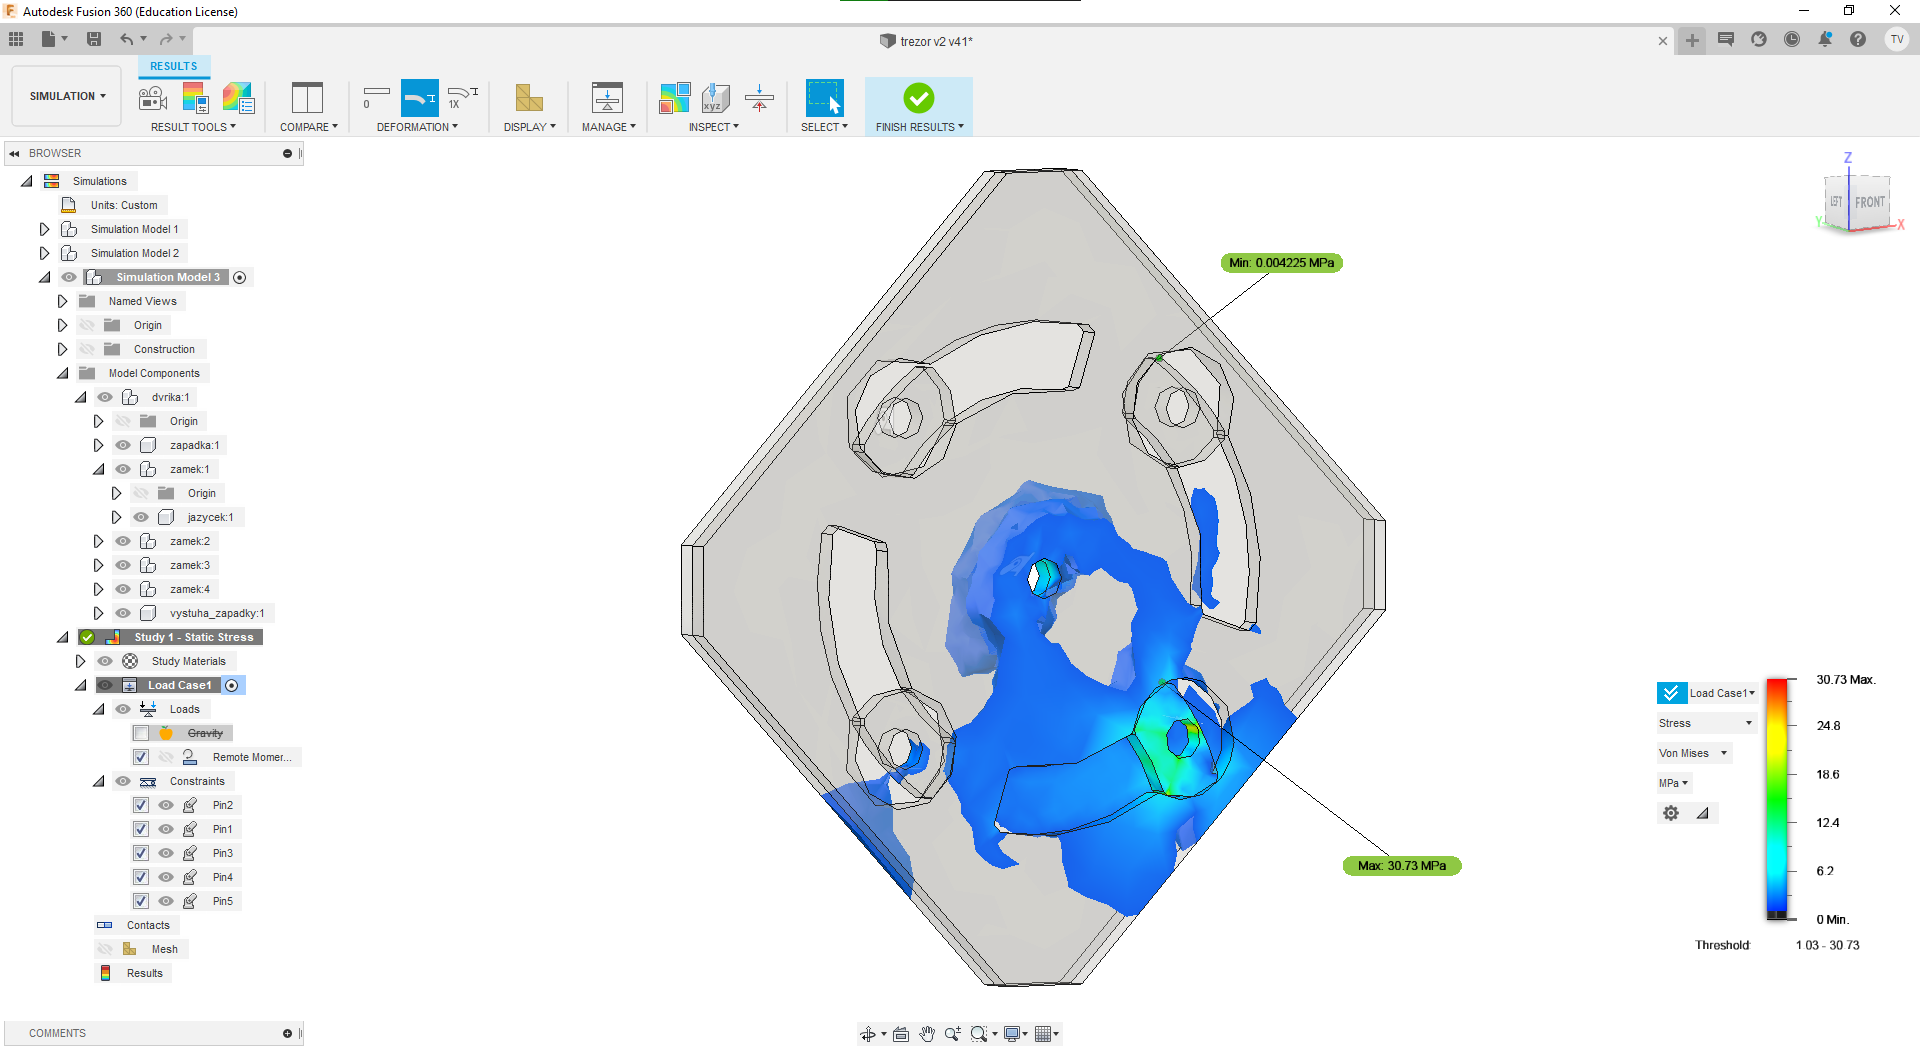
\includegraphics[width=\textwidth]{kapitoly/obrazky/M3/simulace/odolnost_proti_nasilnemu_odemceni_10Nm.png}
    \caption{simulace pokusu o otevření bez předchozího odemčení při kroutícím momentu 10 000 Nmm, zobrazeno jen napětí nad 1 MPa}
    \label{fig:M3-simulace-vytrzeni}
\end{figure}

Ke kompletní simulaci se můžete dostat \href{https://myhub.autodesk360.com/ue2d7aa41/g/shares/SH56a43QTfd62c1cd96843f1e03a0eb48053?viewState=NoIgbgDAdAjCA0IDeAdEAXAngBwKZoC40BlASwFsBXAGwEN1SB7AOzXjVoGdPd1C0ARjABsATlEQItALQBjcbmkAWCMIjSBuWgA5lAM22ilAVgAmMAOyy9%2BBGkYCAVrlnoAkqcIBmAL4gAukA}{zde}
po kliknutí na "Simulation" a "Simulation Model 3". V tabulce napravo se pak můžete přepínat mezi barevným zobrazení několika veličin.

\subparagraph{Kolík}
Kroutící moment který je dřevěný kolík o průměru 6mm schopen přenést. 

\(\tau _M_A_X = 52.3 MPa\)    (\href{https://is.mendelu.cz/eknihovna/opory/zobraz_cast.pl?fit_w=1;cast=9190}{dubové dřevo ve směru vláken při vlhkosti 12 \% })

D = 6

\tau _M_A_X = \frac{M_K}{W_K} \Rightarrow M_K = \tau _MAX * W_K = \sigma _D * \frac{\pi * D^3}{16} 

\(M_K = 52.3 * \frac{\pi * 6^3}{16} = 2 218.16 N*mm \Rightarrow\) a ze simulace že kolík je při namáhání v krutu nejslabším místem \(\Rightarrow\) pro zvýšení odolnosti by bylo 
potřeba zvětšit kolík nebo změnit materiál.